\chapter{Peruuttava haku}

\index{backtracking}
\emph{Peruuttava haku} (\emph{backtracking}) on menetelmä,
jonka avulla voimme käydä järjestelmällisesti kaikki yhdistelmät,
jotka voidaan muodostaa annetuista aineksista.
Peruuttava haku on raa'an voiman algoritmi,
jonka toteutus on yleensä suoraviivainen,
ja menetelmä on käyttökelpoinen silloin,
kun yhdistelmien määrä on niin pieni, että ehdimme käydä kaikki läpi.

Tässä luvussa tutustumme ensin peruuttavan haun algoritmeihin,
jotka käyvät läpi lukujen yhdistelmiä.
Tämän jälkeen näemme, miten peruuttavaa hakua voi käyttää
kahdessa vaikeammassa ongelmassa ja miten hakua voi tehostaa.
Lopuksi toteutamme pelin tekoälyn minimax-algoritmilla,
joka perustuu peruuttavaan hakuun.

\section{Silmukoista rekursioon}

Oletetaan, että haluamme käydä läpi kaikki $n$ luvun yhdistelmät,
joissa jokainen luku on kokonaisluku väliltä $1 \dots m$.
Tällaisia yhdistelmiä on yhteensä $m^n$,
koska kohtia on $n$ ja joka kohdassa luvun voi valita $m$ tavalla.
Esimerkiksi jos $n=3$ ja $m=4$, yhdistelmät ovat
$[1,1,1]$, $[1,1,2]$, $[1,1,3]$, $[1,1,4]$, $[1,2,1]$,
$[1,2,2]$, $[1,2,3]$, $[1,2,4]$, jne.

Jos lukujen määrä $n$ on etukäteen tiedossa, voimme
luoda $n$ sisäkkäistä silmukkaa, joista jokainen käy $m$ lukua läpi.
Esimerkiksi seuraava koodi käy läpi kaikki yhdistelmät
tapauksessa $n=3$:

\begin{code}
for a = 1 to m
    for b = 1 to m
        for c = 1 to m
            print(a,b,c)
\end{code}

Tämä on sinänsä mainio ratkaisu, mutta siinä on yksi ongelma:
lukujen määrä $n$ vaikuttaa silmukoiden määrään.
Jos haluaisimme muuttaa $n$:n arvoa, meidän täytyisi muuttaa
koodin silmukoiden määrää, mikä ei ole hyvä asia.
Peruuttavan haun avulla voimme kuitenkin toteuttaa ratkaisun
rekursiivisesti niin, että sama koodi toimii kaikille $n$:n arvoille.

\subsection{Haun toteuttaminen}

Seuraava rekursiivinen proseduuri \texttt{haku} muodostaa
yhdistelmiä peruuttavan haun avulla.
Parametri $k$ tarkoittaa kohtaa, johon seuraava luku asetetaan.
Jos $k=n$, jokin yhdistelmä on valmistunut, jolloin se tulostetaan.
Muuten haku käy läpi kaikki tavat sijoittaa kohtaan $k$ luku $1 \dots m$
ja jatkaa rekursiivisesti kohtaan $k+1$.
Haku lähtee käyntiin kutsulla \texttt{haku}(0),
ja \texttt{luvut} on $n$-kokoinen taulukko, johon yhdistelmä muodostetaan.

\begin{code}
procedure haku(k)
    if k == n
        print(luvut)
    else
        for i = 1 to m
            luvut[k] = i
            haku(k+1)
\end{code}

Kuva \ref{fig:perhak} näyttää, miten haku lähtee liikkeelle
tapauksessa $n=3$ ja $m=4$.
Merkki "$-$" tarkoittaa lukua, jota ei ole vielä valittu.
Haun ensimmäinen taso valitsee yhdistelmän
ensimmäisen luvun kohtaan $0$.
Tämän valintaan on neljä vaihtoehtoa,
koska mahdolliset luvut ovat $1 \dots 4$,
joten haku haarautuu neljään osaan.
Tämän jälkeen haku jatkaa rekursiivisesti eteenpäin
ja valitsee muihin kohtiin tulevat luvut.

\begin{figure}
\center
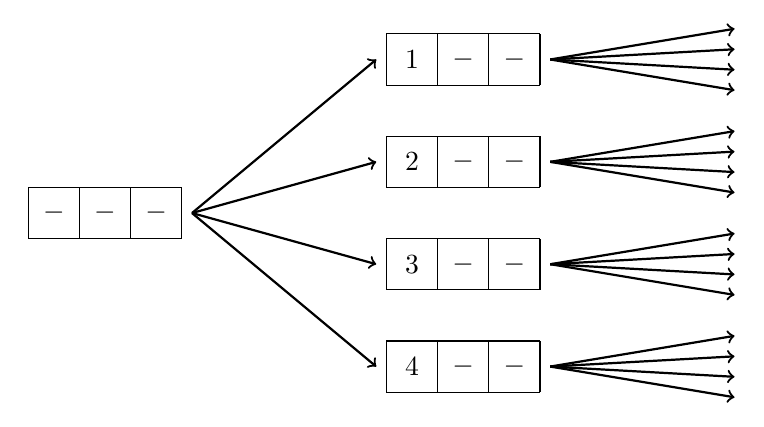
\begin{tikzpicture}[scale=.65]
    \draw (0,0) grid (3,1);
    \foreach \x/\v in {0/-,1/-,2/-} \node at (\x+0.5,0.5) {$\v$};

    \draw (7,-3) grid (10,-2);
    \foreach \x/\v in {0/1,1/-,2/-} \node at (\x+7.5,3.5) {$\v$};
    \draw (7,-1) grid (10,0);
    \foreach \x/\v in {0/2,1/-,2/-} \node at (\x+7.5,1.5) {$\v$};
    \draw (7,1) grid (10,2);
    \foreach \x/\v in {0/3,1/-,2/-} \node at (\x+7.5,-0.5) {$\v$};
    \draw (7,3) grid (10,4);
    \foreach \x/\v in {0/4,1/-,2/-} \node at (\x+7.5,-2.5) {$\v$};

    \draw[->,thick] (3.2,0.5) -- (6.8,3.5);
    \draw[->,thick] (3.2,0.5) -- (6.8,1.5);
    \draw[->,thick] (3.2,0.5) -- (6.8,-0.5);
    \draw[->,thick] (3.2,0.5) -- (6.8,-2.5);
    
    \foreach \y in {3.5,1.5,-0.5,-2.5} \foreach \z in {0.6,0.2,-0.2,-0.6}
        \draw[->,thick] (10.2,\y) -- (13.8,\y+\z);
\end{tikzpicture}
\caption{Yhdistelmien muodostaminen alkaa ($n=3$ ja $m=4$).}
\label{fig:perhak}
\end{figure}

Voimme arvioida algoritmin tehokkuutta laskemalla,
montako kertaa proseduuria \texttt{haku} kutsutaan yhteensä haun aikana.
Proseduuria kutsutaan kerran parametrilla $0$,
$m$ kertaa parametrilla $1$, $m^2$ kertaa parametrilla $2$, jne.,
joten kutsujen määrä on yhteensä
\[
1+m+m^2+\dots+m^n = \frac{m^{n+1}-1}{m-1} = O(m^n).
\]
Tästä näkee, että kutsujen yhteismäärä on samaa luokkaa kuin
viimeisen tason kutsujen määrä.
Viimeisellä tasolla tehdäänkin enemmän kutsuja kuin
kaikilla muilla tasoilla yhteensä.

\subsection{Osajoukkojen läpikäynti}

Tarkastellaan sitten tilannetta,
jossa haluamme käydä läpi kaikki $n$ alkion
joukon \emph{osajoukot}.
Osajoukkoja on yhteensä $2^n$,
koska jokainen alkio joko kuuluu tai ei kuulu osajoukkoon.
Esimerkiksi joukon $\{2,3,5,9\}$ osajoukkoja ovat
$\{2,5\}$ ja $\{3,5,9\}$.

Osoittautuu, että voimme muodostaa osajoukot
käymällä läpi kaikki $n$ luvun yhdistelmät,
joissa jokainen luku on 0 tai 1.
Ideana on, että jokainen yhdistelmän luku kertoo,
kuuluuko tietty alkio osajoukkoon,
Alkio kuuluu osajoukkoon tarkalleen silloin,
kun sen kohdalla on luku 1.
Esimerkiksi kun joukkona on $\{2,3,5,9\}$,
yhdistelmä $[1,0,1,0]$ vastaa
osajoukkoa $\{2,5\}$ ja
yhdistelmä $[0,1,1,1]$ vastaa osajoukkoa $\{3,5,9\}$.

Seuraava koodi näyttää, miten voimme käydä osajoukot
läpi peruuttavan haun avulla.
Proseduuri \texttt{haku} valitsee,
otetaanko kohdassa $k$ oleva alkio mukaan osajoukkoon vai ei,
ja merkitsee tämän tiedon taulukkoon \texttt{valinta}.
Kuten ennenkin, haku lähtee käyntiin kutsulla \texttt{haku}$(0)$.

\begin{code}
procedure haku(k)
    if k == n
        // käsittele osajoukko
    else
        for i = 0 to 1
            valinta[k] = i
            haku(k+1)
\end{code}

\subsection{Permutaatioiden läpikäynti}

Peruuttavan haun avulla voimme myös käydä läpi joukon
\emph{permutaatiot} eli erilaiset järjestykset.
Kun joukossa on $n$ alkiota, siitä voidaan muodostaa
kaikkiaan $n!$ permutaatiota.
Esimerkiksi joukon $\{1,2,3,4\}$ permutaatioita ovat
$\{2,4,1,3\}$ ja $\{4,3,1,2\}$.

Tässä tilanteessa haluamme käydä läpi $n$ luvun yhdistelmiä,
joissa jokainen luku on väliltä $1 \dots n$
ja lisäksi mikään luku ei toistu.
Saamme tämän aikaan lisäämällä hakuun uuden taulukon
\texttt{mukana}, joka kertoo, onko tietty luku jo mukana.
Joka vaiheessa haku valitsee yhdistelmään vain sellaisia lukuja,
joita ei ole valittu siihen aiemmin.

\begin{code}
procedure haku(k)
    if k == n
        print(luvut)
    else
        for i = 1 to n
            if not mukana[i]
                mukana[i] = true
                luvut[k] = i
                haku(k+1)
                mukana[i] = false
\end{code}

\section{Esimerkkejä}

Käymme seuraavaksi läpi kaksi vaativampaa esimerkkiä
peruuttavan haun soveltamisesta.
Ratkaisemme ensin shakkiin liittyvän ongelman,
ja tämän jälkeen etsimme parhaan tavan
työtehtävien jakamiseen.
Molemmissa sovelluksissa näemme myös,
miten peruuttavaa hakua voi tehostaa.

\subsection{Kuningatarongelma}

Tehtävämme on laskea, monellako tavalla
$n \times n$ -shakkilaudalle voidaan asettaa $n$ kuningatarta
niin, etteivät mitkään kaksi kuningatarta uhkaa toisiaan.
Shakissa kuningattaret voivat uhata toisiaan
vaaka-, pysty- tai vinosuuntaisesti.
Esimerkiksi tapauksessa $n=4$ mahdollisia sijoitustapoja on kaksi,
jotka on esitetty kuvassa \ref{fig:kuning}.

\begin{figure}[h]
\center
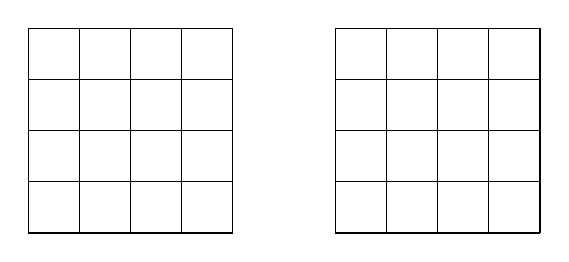
\begin{tikzpicture}[scale=.65]
  \begin{scope}
    \draw (0, 0) grid (4, 4);
    \node at (1.5,3.5) {$\symqueen$};
    \node at (3.5,2.5) {$\symqueen$};
    \node at (0.5,1.5) {$\symqueen$};
    \node at (2.5,0.5) {$\symqueen$};

    \draw (6, 0) grid (10, 4);
    \node at (6+2.5,3.5) {$\symqueen$};
    \node at (6+0.5,2.5) {$\symqueen$};
    \node at (6+3.5,1.5) {$\symqueen$};
    \node at (6+1.5,0.5) {$\symqueen$};
  \end{scope}
\end{tikzpicture}
\caption{Kuningatarongelman ratkaisut tapauksessa $n=4$.}
\label{fig:kuning}
\end{figure}

Voimme ratkaista tehtävän toteuttamalla algoritmin,
joka käy laudan läpi ylhäältä alaspäin ja asettaa yhden kuningattaren
jokaiselle riville.
Kuva \ref{fig:hakupuu} esittää haun toimintaa tapauksessa $n=4$.
Ensimmäisen rivin kuningatar voidaan asettaa mihin tahansa sarakkeeseen,
mutta seuraavilla riveillä aiemmat valinnat rajoittavat hakua.
Kuvassa näkyy toisen kuningattaren sijoittaminen,
kun ensimmäinen kuningatar on toisessa sarakkeessa.
Tällöin ainoa vaihtoehto on, että toinen kuningatar on viimeisessä sarakkeessa,
koska kaikissa muissa tapauksissa kuningattaret uhkaisivat toisiaan.


\begin{figure}
\center
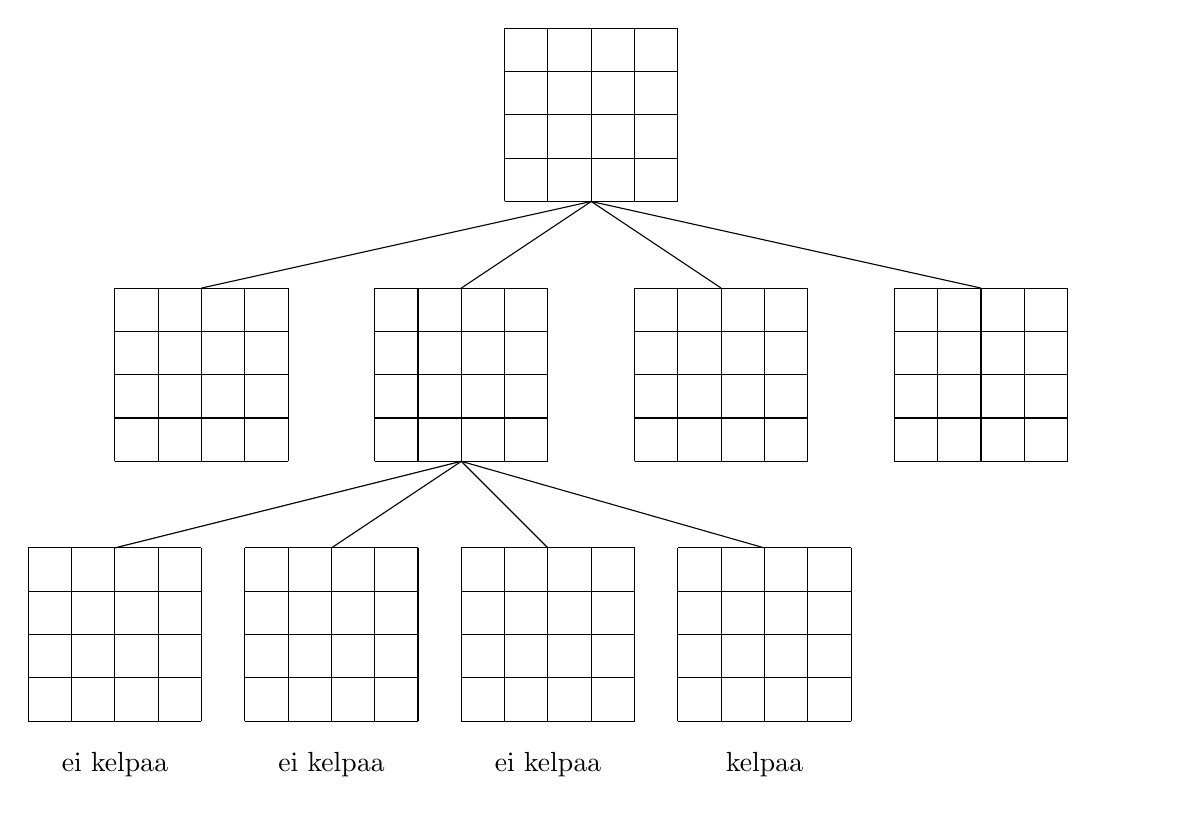
\begin{tikzpicture}[scale=.55]
  \begin{scope}
    \draw (0, 0) grid (4, 4);

    \draw (-9, -6) grid (-5, -2);
    \draw (-3, -6) grid (1, -2);
    \draw (3, -6) grid (7, -2);
    \draw (9, -6) grid (13, -2);

    \node at (-9+0.5,-3+0.5) {$\symqueen$};
    \node at (-3+1+0.5,-3+0.5) {$\symqueen$};
    \node at (3+2+0.5,-3+0.5) {$\symqueen$};
    \node at (9+3+0.5,-3+0.5) {$\symqueen$};

    \draw (2,0) -- (-7,-2);
    \draw (2,0) -- (-1,-2);
    \draw (2,0) -- (5,-2);
    \draw (2,0) -- (11,-2);

    \draw (-11, -12) grid (-7, -8);
    \draw (-6, -12) grid (-2, -8);
    \draw (-1, -12) grid (3, -8);
    \draw (4, -12) grid (8, -8);
    \draw[white] (11, -12) grid (15, -8);
    \node at (-11+1+0.5,-9+0.5) {$\symqueen$};
    \node at (-6+1+0.5,-9+0.5) {$\symqueen$};
    \node at (-1+1+0.5,-9+0.5) {$\symqueen$};
    \node at (4+1+0.5,-9+0.5) {$\symqueen$};
    \node at (-11+0+0.5,-10+0.5) {$\symqueen$};
    \node at (-6+1+0.5,-10+0.5) {$\symqueen$};
    \node at (-1+2+0.5,-10+0.5) {$\symqueen$};
    \node at (4+3+0.5,-10+0.5) {$\symqueen$};

    \draw (-1,-6) -- (-9,-8);
    \draw (-1,-6) -- (-4,-8);
    \draw (-1,-6) -- (1,-8);
    \draw (-1,-6) -- (6,-8);
    
    \node at (-9,-13) {ei kelpaa};
    \node at (-4,-13) {ei kelpaa};
    \node at (1,-13) {ei kelpaa};
    \node at (6,-13) {kelpaa};    
  \end{scope}
\end{tikzpicture}
\caption{Peruuttavan haun toiminta kuningatarongelmassa.}
\label{fig:hakupuu}
\end{figure}


Seuraava proseduuri \texttt{haku} esittää peruuttavan haun algoritmin,
joka laskee kuningatarongelman ratkaisut:

\begin{code}
procedure haku(y)
    if y == n
        laskuri += 1
    else
        for x = 0 to n-1
            if voi_sijoittaa(y,x)
                kohta[y] = x
                haku(y+1)
\end{code}

Oletamme, että laudan rivit ja sarakkeet on numeroitu $0 \dots n-1$.
Parametri $y$ kertoo, mille riville seuraava kuningatar tulee sijoittaa,
ja haku lähtee käyntiin kutsulla \texttt{haku}$(0)$.
Jos rivinä on $n$, kaikki kuningattaret on jo sijoitettu,
joten yksi ratkaisu on löytynyt.
Muuten suoritetaan silmukka, joka käy läpi mahdolliset sarakkeet
muuttujan $x$ avulla.
Jos kuningatar voidaan sijoittaa sarakkeeseen $x$
eli se ei uhkaa mitään aiemmin sijoitettua kuningatarta,
merkitään taulukkoon \texttt{kohta},
että kuningatar $y$ on sarakkeessa $x$,
ja haku jatkuu eteenpäin rekursiivisesti.

Lisäksi täytyy toteuttaa funktio \texttt{voi\_sijoittaa},
joka tutkii, voidaanko uusi kuningatar sijoittaa
rivin $y$ sarakkeeseen $x$.
Tämä voidaan selvittää taulukon \texttt{kohta} avulla näin:

\begin{code}
function voi_sijoittaa(y,x)
    for i = 0 to y-1
        if kohta[i] == x
            return false
        if abs(i-y) == abs(kohta[i]-x)
            return false
    return true
\end{code}

Funktio käy läpi kaikki aiemmin sijoitetut kuningattaret.
Jos aiemmin sijoitettu kuningatar olisi samassa sarakkeessa
(ensimmäinen ehto) tai samalla vinorivillä (toinen ehto)
kuin uusi kuningatar, tällaista sijoitusta ei voida tehdä
ja funktio palauttaa \texttt{false}.
Jos taas mikään aiempi kuningatar ei uhkaa uutta kuningatarta,
funktio palauttaa \texttt{true}.
Huomaa jälkimmäisessä ehdossa kätevä tapa tarkastaa
itseisarvon (funktio \texttt{abs}) avulla,
ovatko kuningattaret samalla vinorivillä.
Kuningattaret ovat samalla vinorivillä tarkalleen silloin,
kun niiden vaaka- ja pystysuuntaiset erot ovat samat.

\begin{table}
\center
\begin{tabular}{rr}
laudan koko $n$ & ratkaisujen määrä \\
\hline
1 & 1 \\
2 & 0 \\
3 & 0 \\
4 & 2 \\
5 & 10 \\
6 & 4 \\
7 & 40 \\
8 & 92 \\
9 & 352 \\
10 & 724 \\
\end{tabular}
\caption{Kuningatarongelman ratkaisujen määriä.}
\label{tab:kuning}
\end{table}

Nyt meillä on valmis algoritmi, jonka avulla voimme
käydä läpi kuningatarongelman ratkaisuja.
Taulukko \ref{tab:kuning} näyttää ratkaisujen määrät
tapauksissa $n=1 \dots 10$.
Algoritmi selvittää nämä tapaukset salamannopeasti,
mutta suuremmilla $n$:n arvoilla algoritmi alkaa viedä paljon aikaa.
Syynä tähän on, että kuningatarten sijoitustapojen
määrä kasvaa \emph{eksponentiaalisesti}
eli räjähdysmäisen nopeasti.
Esimerkiksi tapauksessa $n=20$ erilaisia ratkaisuja on jo yli 39 miljardia.

\index{symmetria}
Voimme kuitenkin koettaa nopeuttaa algoritmia parantamalla
sen toteutusta.
Yksi helppo tehostus on hyödyntää \emph{symmetriaa}.
Jokaista kuningatar\-ongelman ratkaisua vastaa toinen ratkaisu,
joka saadaan peilaamalla ratkaisu vaakasuuntaisesti.
Esimerkiksi kuvassa \ref{fig:kuning} ratkaisut voidaan muuttaa
toisikseen peilaamalla.
Tämän havainnon ansiosta voimme puolittaa algoritmin suoritusajan
lisäämällä vaatimuksen, että ensimmäinen kuningatar asetetaan
laudan vasempaan puoliskoon, ja kertomalla lopuksi vastauksen kahdella.
Jos laudan koko on pariton, täytyy vielä käsitellä erikseen tapaus,
jossa ensimmäinen kuningatar sijoitetaan keskisarakkeeseen.

Toinen mahdollinen tehostus olisi toteuttaa funktio
\texttt{voi\_sijoittaa} paremmin.
Tällä hetkellä se käy läpi kaikki aiemmin sijoitetut kuningattaret
ja vie aikaa $O(n)$, mutta funktio on mahdollista toteuttaa myös
ajassa $O(1)$ ottamalla käyttöön uusia aputaulukoita, joissa on tietoa,
mitkä sarakkeet ja vinorivit ovat uhattuina.
Tämä tehostus on kuitenkin vaikeampi toteuttaa kuin symmetristen ratkaisujen karsinta.

Kuningatarongelma on kuitenkin pohjimmiltaan vaikea ongelma,
eikä sen ratkaisuun tunneta mitään oleellisesti raakaa voimaa
parempaa tapaa.
Tällä hetkellä suurin tapaus, jonka ratkaisu tunnetaan, on $n=27$.
Tämän tapauksen käsittely vei aikaa noin vuoden laskentaklusterilla,
jossa oli suuri määrä rinnakkain laskevia
suorittimia\footnote{27-Queens Puzzle: Massively Parellel Enumeration and Solution Counting.
\url{https://github.com/preusser/q27}}.

\subsection{Työtehtävien jakaminen}

Tarkastellaan tilannetta, jossa on $n$ työtehtävää ja $n$ työntekijää.
Tehtävät tulee jakaa työntekijöille niin,
että jokainen työntekijä suorittaa tarkalleen yhden työtehtävän.
Jokaisesta työtehtävästä tiedetään,
paljonko sen suorittaminen maksaa kullakin työntekijällä,
ja tavoitteena on etsiä ratkaisu, jossa kokonaishinta on pienin mahdollinen.

\begin{figure}
\center
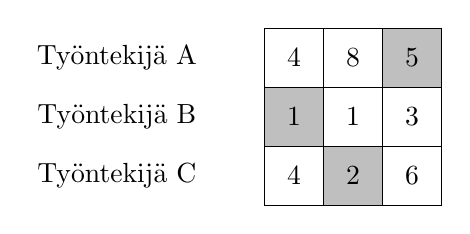
\begin{tikzpicture}[scale=0.75]
\fill[color=lightgray] (0,1) rectangle (1,2);
\fill[color=lightgray] (1,0) rectangle (2,1);
\fill[color=lightgray] (2,2) rectangle (3,3);
\draw (0,0) grid (3,3);
\node at (0.5,0.5) {$4$};
\node at (1.5,0.5) {$2$};
\node at (2.5,0.5) {$6$};
\node at (0.5,1.5) {$1$};
\node at (1.5,1.5) {$1$};
\node at (2.5,1.5) {$3$};
\node at (0.5,2.5) {$4$};
\node at (1.5,2.5) {$8$};
\node at (2.5,2.5) {$5$};
\node at (-2.5,2.5) {Työntekijä A};
\node at (-2.5,1.5) {Työntekijä B};
\node at (-2.5,0.5) {Työntekijä C};
\end{tikzpicture}
\caption{Optimaalinen tapa jakaa työtehtävät.}
\label{fig:tyoteh}
\end{figure}

Kuvassa \ref{fig:tyoteh} on esimerkki tilanteesta, jossa $n=3$.
Tässä optimaalinen tapa jakaa työtehtävät on,
että B suorittaa ensimmäisen työtehtävän,
C suorittaa toisen työtehtävän ja
A suorittaa kolmannen työtehtävän.
Tämän ratkaisun kustannus on $1+2+5=8$.

Oletamme, että työtehtävät ja työntekijät on numeroitu
$0 \dots n-1$ ja voimme lukea taulukosta \texttt{hinta}$[a][b]$,
paljonko työtehtävän $a$ suorittaminen maksaa
työntekijällä $b$.
Toteutamme peruuttavan haun algoritmin,
joka käy läpi työtehtävät järjestyksessä
ja valitsee jokaiselle työntekijän.

Seuraava proseduuri \texttt{haku} saa kaksi parametria:
$k$ on seuraavaksi käsitel\-tävä työtehtävä ja
$h$ on tähän mennessä muodostunut hinta.
Haku lähtee käyntiin kutsulla \texttt{haku}$(0,0)$.
Taulukko \texttt{mukana} pitää kirjaa,
mitkä työntekijät on jo valittu,
ja muuttujassa $p$ on yhteishinta
parhaassa tähän mennessä löytyneessä ratkaisussa.
Ennen hakua muuttujan $p$ arvona on $\infty$,
koska mi\-tään ratkaisua ei ole vielä olemassa.

\begin{code}
procedure haku(k,h)
    if k == n
        p = min(p,h)
    else
        for i = 0 to n-1
            if not mukana[i]
                mukana[i] = true
                haku(k+1,h+hinta[k][i])
                mukana[i] = false
\end{code}

Tämä on toimiva peruuttavan haun algoritmi,
ja haun päätteeksi muuttujassa $p$ on
parhaan ratkaisun yhteishinta.
Algoritmi on kuitenkin hidas, koska se käy aina läpi
kaikki $n!$ mahdollista ratkaisua.
Koska haluamme vain löytää parhaan ratkaisun emmekä
käydä läpi kaikkia ratkaisuja,
pystymme tehostamaan algoritmia lisäämään siihen ehdon,
joka lopettaa ratkaisun muodostamisen,
jos siitä ei voi tulla aiempaa parempi.

\index{branch and bound}
Testaamme seuraavaksi algoritmia tapauksella, jossa $n=20$ ja jokainen
taulukossa \texttt{hinta} oleva arvo on satunnainen
kokonaisluku välillä $1 \dots 100$.
Tässä tapauksessa edellä kuvattu algoritmi kävisi läpi 
\[20! = 2432902008176640000
\]
eri ratkaisua, mikä veisi aikaa \emph{satoja vuosia}.
Jotta voimme ratkaista tapauksen,
meidän täytyy parantaa algoritmia niin,
että se ei käy läpi kaikkia ratkaisuja
mutta löytää kuitenkin parhaan ratkaisun.
Tässä avuksi tulee tekniikka, josta käytetään usein nimeä
\emph{branch and bound}.
Siinä ideana on tehostaa peruuttavaa hakua
vähentämällä tutkittavien ratkaisujen määrää
sopivien ylä- ja alarajojen avulla.

Keskeinen havainto on, että voimme rajoittaa hakua muuttujan
$p$ avulla. Tässä muuttujassa on joka hetkellä
tähän mennessä parhaan löydetyn ratkaisun yhteishinta,
joten tämä on \emph{yläraja} sille, kuinka suuri parhaan ratkaisun
yhteishinta voi olla.
Toisaalta muuttujassa $h$ on muodosteilla olevan ratkaisun
hinta tässä vaiheessa, joka on \emph{alaraja} yhteishinnalle.
Jos $h \ge p$, muodosteilla olevasta ratkaisusta ei
voi tulla aiempaa parempaa. Voimmekin lisätä algoritmin alkuun
seuraavan tarkastuksen:

\begin{code}
procedure haku(k,h)
    if h >= p
        return
    ...
\end{code}

Tämän ansiosta ratkaisun muodostaminen päättyy heti,
jos sen hinta on yhtä suuri tai suurempi kuin parhaan
tiedossa olevan ratkaisun hinta.
Tämän tehostuksen avulla saamme ratkaistua
muodostamamme tapauksen testikoneella 152 sekunnissa.
Tämä on hieno saavutus, koska alkuperäinen algoritmi
ei kyennyt ratkaisemaan tapausta lainkaan.

Voimme kuitenkin tehostaa algoritmia vielä lisää
laskemalla tarkemman arvion alarajalle.
Muodosteilla olevan ratkaisun hinta on varmasti ainakin $h$,
mutta voimme lisäksi arvioida, paljonko myöhemmin valittavat
työntekijät lisäävät kustannusta:

\begin{code}
procedure haku(k,h)
    if h+arvio(k) >= p
        return
    ...
\end{code}

Tässä funktion \texttt{arvio} tulee antaa jokin arvio,
paljonko ainakin maksaa suorittaa jäljellä olevat työtehtävät $k \dots n-1$.
Yksi kätevä tapa saada arvio on käydä läpi jäljellä olevat
työtehtävät ja valita jokaisen tekijäksi \emph{halvin} työntekijä välittämättä
siitä, onko kyseinen työntekijä mahdollisesti valittu aiemmin.
Tämä antaa alarajan sille, paljonko kustannuksia on ainakin vielä tiedossa.
Tämän tehostuksen jälkeen tapauksen $n=20$ käsittely vie
testikoneella vain 7 sekuntia.
Paremman alarajan ansiosta saimme siis algoritmin
vielä noin 20 kertaa nopeammaksi verrattuna edelliseen versioon.

\section{Pelin tekoäly}

Peruuttavan haun avulla voi myös toteuttaa tekoälyn kahden pelaajan peliin,
kuten ristinollaan tai shakkiin.
Tällaisen tekoälyn täytyy pystyä päättämään,
miten toimia annetussa pelin tilanteessa.
Ideana on luoda haku, joka käy läpi
järjestelmällisesti mahdollisia siirtoja,
joita pelaajat voivat tehdä.

\subsection{Minimax-algoritmi}

\index{minimax-algoritmi}
\emph{Minimax-algoritmi} on peruuttavaan hakuun perustuva algoritmi,
joka valitsee tekoälyn siirron pelissä.
Se käy läpi pelinkulkuja tiettyyn syvyyteen asti,
arvioi pelitilanteet ja valitsee siirron,
joka takaa mahdollisimman hyvältä vaikuttavan tuloksen.
Algoritmin nimi tulee siitä, että se vuorotellen
\emph{minimoi} ja \emph{maksimoi} tulosta puun kerroksissa.

\begin{figure}
\center
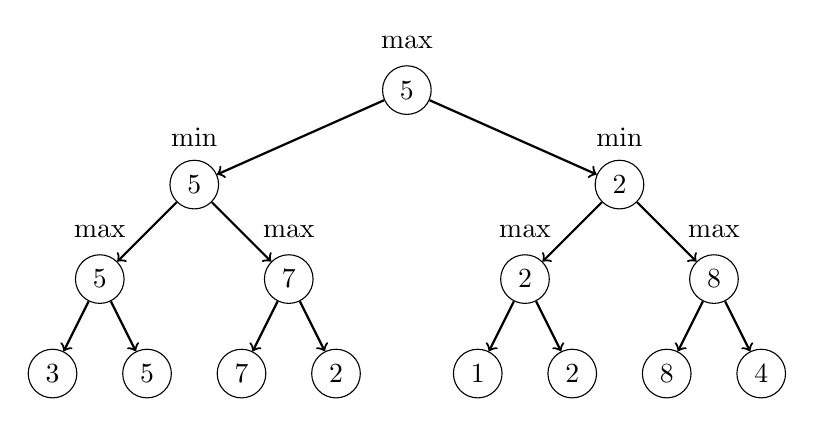
\begin{tikzpicture}[scale=0.6]
\node[draw, circle] (1) at (0,0) {$5$};
\node[draw, circle] (2) at (-4.5,-2) {$5$};
\node[draw, circle] (3) at (4.5,-2) {$2$};
\node[draw, circle] (4) at (-6.5,-4) {$5$};
\node[draw, circle] (5) at (-2.5,-4) {$7$};
\node[draw, circle] (6) at (2.5,-4) {$2$};
\node[draw, circle] (7) at (6.5,-4) {$8$};
\node[draw, circle] (8) at (-7.5,-6) {$3$};
\node[draw, circle] (9) at (-5.5,-6) {$5$};
\node[draw, circle] (10) at (-3.5,-6) {$7$};
\node[draw, circle] (11) at (-1.5,-6) {$2$};
\node[draw, circle] (12) at (1.5,-6) {$1$};
\node[draw, circle] (13) at (3.5,-6) {$2$};
\node[draw, circle] (14) at (5.5,-6) {$8$};
\node[draw, circle] (15) at (7.5,-6) {$4$};
\path[draw,thick,->] (1) -- (2);
\path[draw,thick,->] (1) -- (3);
\path[draw,thick,->] (2) -- (4);
\path[draw,thick,->] (2) -- (5);
\path[draw,thick,->] (3) -- (6);
\path[draw,thick,->] (3) -- (7);
\path[draw,thick,->] (4) -- (8);
\path[draw,thick,->] (4) -- (9);
\path[draw,thick,->] (5) -- (10);
\path[draw,thick,->] (5) -- (11);
\path[draw,thick,->] (6) -- (12);
\path[draw,thick,->] (6) -- (13);
\path[draw,thick,->] (7) -- (14);
\path[draw,thick,->] (7) -- (15);
\node at (0,1) {max};
\node at (-4.5,-1) {min};
\node at (4.5,-1) {min};
\node at (-6.5,-3) {max};
\node at (-2.5,-3) {max};
\node at (2.5,-3) {max};
\node at (6.5,-3) {max};
\end{tikzpicture}
\caption{Esimerkki minimax-algoritmin toiminnasta.}
\label{fig:minmax}
\end{figure}

Kuvassa \ref{fig:minmax} on esimerkki algoritmin toiminnasta,
kun hakusyvyytenä on kolme tasoa ja
joka tilanteessa on kaksi mahdollista siirtoa.
Puun juuressa oleva solmu vastaa nykyistä pelitilannetta,
jossa tekoälyn täytyy päättää seuraava siirto,
ja jokainen askel puussa alaspäin tarkoittaa yhtä siirtoa.
Tässä tekoäly tutkii, mitä kaikkea voi tapahtua,
kun se siirtää ensin itse, sitten vastustaja siirtää,
ja sitten se siirtää uudestaan.
Puun alimmalla tasolla on jokaisen
kolmen siirron päässä olevan pelitilanteen \emph{hyvyys}
eli tekoälyn arvio,
kuinka hyvä kyseinen tilanne on sen itsensä kannalta.

Tekoäly valitsee aina siirron,
joka on mahdollisimman hyvä sen itsensä kannalta.
Toisaalta tekoäly olettaa, että vastustaja valitsee siirron,
joka on mahdollisimman huono tekoälyn kannalta.
Niinpä joka toisella tasolla solmuissa on maksimi lasten arvoista
ja joka toisella tasolla minimi.
Tässä esimerkissä tekoäly tekee siirron,
joka takaa, että kolmen siirron päästä pelitilanteen hyvyys on ainakin 5
riippumatta vastustajan toimista.

Tekoälyn pelitaito riippuu kahdesta asiasta:
(1) montako tasoa alemmas se tutkii puuta ja
(2) miten hyvin se osaa arvioida pohjalla olevia pelitilanteita.
Mitä syvemmälle haku jatkuu, sitä paremmin tekoäly pelaa,
koska se saa enemmän tietoa pelinkuluista,
mutta sitä kauemmin vie, ennen kuin tekoäly tekee päätöksen.
Pelitilanteen arviointi puolestaan vaatii tietoa pelattavasta pelistä.
Esimerkiksi shakissa pelitilannetta voi arvioida tutkimalla,
mitä nappuloita itsellä ja vastustajalla on jäljellä.

\subsection{Alfa-beeta-karsinta}

\begin{figure}
\center
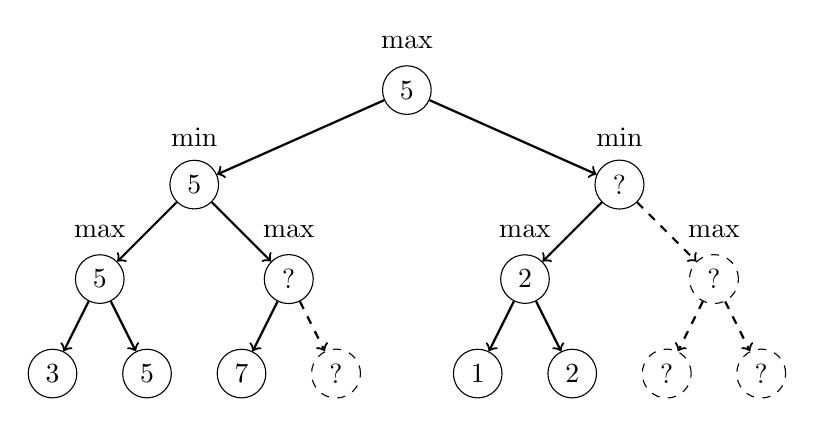
\begin{tikzpicture}[scale=0.6]
\node[draw, circle] (1) at (0,0) {$5$};
\node[draw, circle] (2) at (-4.5,-2) {$5$};
\node[draw, circle] (3) at (4.5,-2) {$?$};
\node[draw, circle] (4) at (-6.5,-4) {$5$};
\node[draw, circle] (5) at (-2.5,-4) {$?$};
\node[draw, circle] (6) at (2.5,-4) {$2$};
\node[draw, circle, dashed] (7) at (6.5,-4) {$?$};
\node[draw, circle] (8) at (-7.5,-6) {$3$};
\node[draw, circle] (9) at (-5.5,-6) {$5$};
\node[draw, circle] (10) at (-3.5,-6) {$7$};
\node[draw, circle, dashed] (11) at (-1.5,-6) {$?$};
\node[draw, circle] (12) at (1.5,-6) {$1$};
\node[draw, circle] (13) at (3.5,-6) {$2$};
\node[draw, circle, dashed] (14) at (5.5,-6) {$?$};
\node[draw, circle, dashed] (15) at (7.5,-6) {$?$};
\path[draw,thick,->] (1) -- (2);
\path[draw,thick,->] (1) -- (3);
\path[draw,thick,->] (2) -- (4);
\path[draw,thick,->] (2) -- (5);
\path[draw,thick,->] (3) -- (6);
\path[draw,thick,->,dashed] (3) -- (7);
\path[draw,thick,->] (4) -- (8);
\path[draw,thick,->] (4) -- (9);
\path[draw,thick,->] (5) -- (10);
\path[draw,thick,->,dashed] (5) -- (11);
\path[draw,thick,->] (6) -- (12);
\path[draw,thick,->] (6) -- (13);
\path[draw,thick,->,dashed] (7) -- (14);
\path[draw,thick,->,dashed] (7) -- (15);
\node at (0,1) {max};
\node at (-4.5,-1) {min};
\node at (4.5,-1) {min};
\node at (-6.5,-3) {max};
\node at (-2.5,-3) {max};
\node at (2.5,-3) {max};
\node at (6.5,-3) {max};
\end{tikzpicture}
\caption{Alfa-beeta-karsinnan vaikutus.}
\label{fig:alfbet}
\end{figure}

\index{alfa-beeta-karsinta}
Minimax-algoritmin toimintaa on mahdollista tehostaa
alfa-beeta-karsinnalla, joka jättää puun osia tutkimatta,
jos on selvää, että ne eivät voi vaikuttaa tekoälyn valintaan.
Tämä muistuttaa aiemmin peruuttavan haun yhteydessä
hyödyntämäämme branch and bound -tekniikaa.

Kuva \ref{fig:alfbet} näyttää, kuinka alfa-beeta-karsinta
onnistuu tehostamaan hakua esimerkkitilanteessamme.
Katkoviivoilla esitetyt puun osat ovat sellaisia,
joita ei ole tarpeen tutkia, koska ne eivät voisi vaikuttaa
ylempänä puussa olevaan osittain laskettuun minimiin tai maksimiin.

Kun tekoäly saapuu vasemmassa haarassa solmuun,
jonka arvona on 7, sen ei enää tarvitse tutkia muita
vasemman haaran solmuja. Tämä johtuu siitä, että tekoäly
tietää jo tässä vaiheessa, että vasemman haaran minimi
on enintään 5. Niinpä sen ei tarvitse laskea maksimia luvusta
7 ja jostain toisesta luvusta, koska tämä ei voisi muuttaa minimiä.

Kun sitten oikeassa haarassa tekoäly on laskenut
toiseksi alimmalla tasolla olevaan solmuun
maksimin 2, sen ei enää tarvitse tutkia muita oikean haaran solmuja.
Tämä johtuu siitä, että juuren maksimi on ainakin 5 ja
oikeassa haarassa valittaisiin minimi luvusta 2 ja jostain toisesta luvusta,
mikä ei voisi kasvattaa juuressa olevaa maksimia.
